\chapter{Implementation}

\section{Software}

\subsection{OpenVPN}
% By default, point-to-point, but since the version 2.0 can be configured in server mode, hence being able to manage hundreds of clients.

\lstset{language=c}
\lstset{commentstyle=\color{colComments}\textit,
float=hbp,%
basicstyle=\ttfamily\footnotesize, %
identifierstyle=\color{colIdentifier}, %
keywordstyle=\color{colKeys}, %
stringstyle=\color{colString}, %
columns=flexible, %
tabsize=2, %
extendedchars=true, %
showspaces=false, %
showstringspaces=false, %
numbers=left, %
numberstyle=\tiny, %
breaklines=true, %
breakautoindent=true, %
captionpos=b}
\begin{lstlisting}[caption=openvpn compress then encrypt -- sample from \texttt{forward.c}, label=list:]
/* Compress, fragment, encrypt and HMAC-sign an outgoing packet. */
void encrypt_sign (struct context *c, bool comp_frag)
{
	struct context_buffers *b = c->c2.buffers;
	const uint8_t *orig_buf = c->c2.buf.data;

	if (comp_frag){
	/* Compress the packet. */
		if (lzo_defined (&c->c2.lzo_compwork))
			lzo_compress (&c->c2.buf, b->lzo_compress_buf, &c->c2.lzo_compwork, &c->c2.frame);
	/* Fragment the packet. */
		if (c->c2.fragment)
			fragment_outgoing (c->c2.fragment, &c->c2.buf, &c->c2.frame_fragment);
	}

  /* Encrypt the packet and write an optional HMAC signature. */
	openvpn_encrypt (&c->c2.buf, b->encrypt_buf, &c->c2.crypto_options, &c->c2.frame);
}
\end{lstlisting}

\begin{figure}[ht]
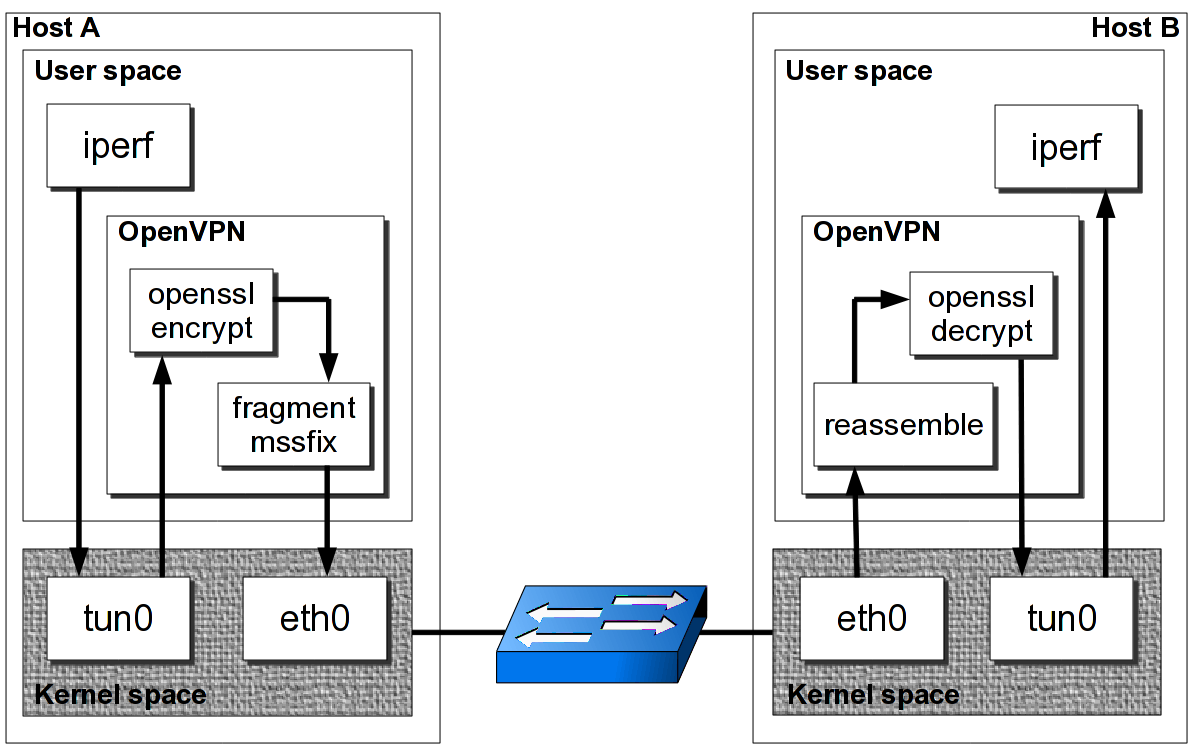
\includegraphics[width=\textwidth]{OpenVPN-packetflow}
\caption{OpenVPN packet flow as advertized on the openVPN wiki.}
\label{fig:openvpn-packet-flow}
\end{figure}

\subsection{OpenSSL}
% Talk about the debug flags in the compilation and show it has close to none impact on the performance (using openssl speed. openssl speed is a relevant test because openssl uses 100% of the CPU, hence maximizing the potential performance reduction.)

It is to be noted that the present work uses an implementation with all the debug flags activated.
If it does have an impact on the performance, it is minimal: in the worst case of the benchmark, the throughput drops only by 2.4\%.
Moreover, the benchmark maximizes this difference by doing only OpenSSL operations.
When OpenSSL will have to share the CPU with other applications, the loss will be even less noticeable.
\begin{figure}[ht]
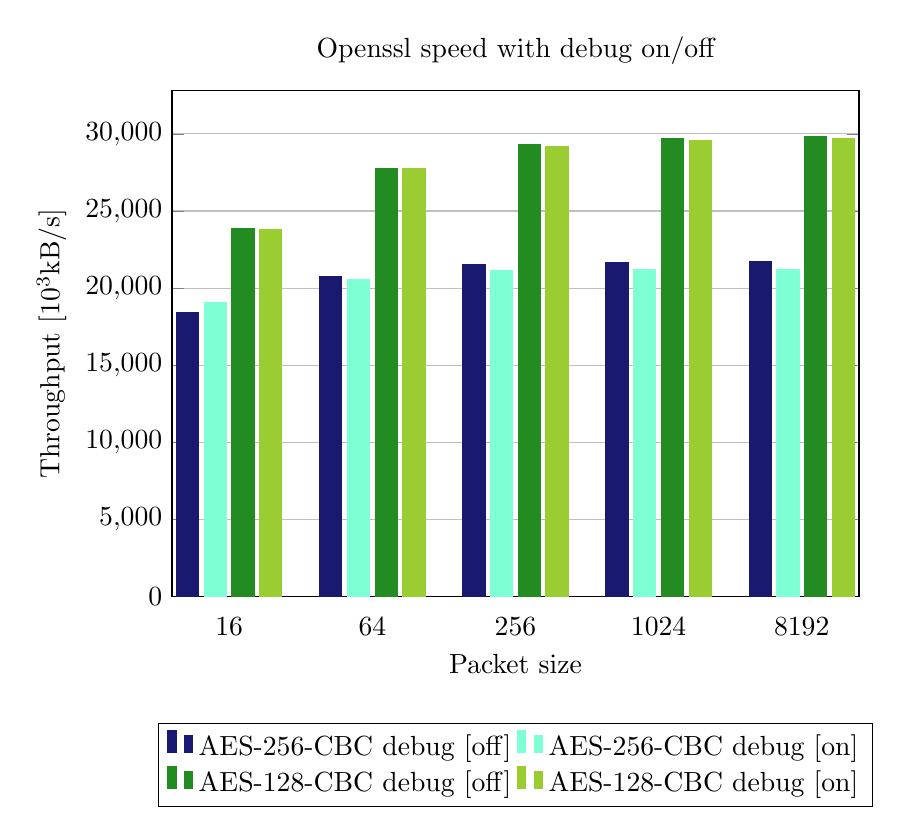
\begin{tikzpicture}
\begin{axis}[
		title = {Openssl speed with debug on/off},
        width  = 0.85*\textwidth,
        height = 8cm,
        major x tick style = transparent,
        ybar,
        bar width=8pt,
        ymajorgrids = true,
        ylabel = {Throughput [$10^3$kB/s]},
        xlabel = {Packet size},
        ymin=0,
        symbolic x coords={16,64,256,1024,8192},
        xtick = data,
        scaled y ticks = false,%Disable the *10^4 exponent applied to all y axis markings.
        legend style={at={(0.5,-0.25)},	anchor=north,legend columns=2},
        enlarge x limits=0.1,
    ]
\addplot[style={MidnightBlue,fill=MidnightBlue,mark=none}]
	coordinates {(16,18400.60) (64,20750.61) (256,21507.33) (1024,21681.15) (8192,21725.18)};
	\label{aes-256-cbc-dbg-off}

\addplot[style={Aquamarine,fill=Aquamarine,mark=none}]
	coordinates {(16,19091.65) (64,20579.24) (256,21106.60) (1024,21216.26) (8192,21203.63)};
	\label{aes-256-cbc-dbg-on}

\addplot[style={ForestGreen,fill=ForestGreen,mark=none}]
	coordinates {(16,23882.41) (64,27781.80) (256,29285.63) (1024,29692.25) (8192,29807.96)};
	\label{aes-128-cbc-dbg-off}

\addplot[style={YellowGreen,fill=YellowGreen,mark=none}]
	coordinates {(16,23806.36) (64,27728.96) (256,29181.70) (1024,29573.46) (8192,29687.81)};
	\label{aes-128-cbc-dbg-on}

\legend{AES-256-CBC debug [off], AES-256-CBC debug [on], AES-128-CBC debug [off], AES-128-CBC debug [on]}
\end{axis}
\end{tikzpicture}
\label{fig:openssl-speed-dbg-on-off}
\caption{Software benchmark of Openssl speed for AES mode CBC, with 128- and 256-bit keys, debugging flags (de)activated at compilation (\texttt{-fno-inline -g -marm}).}
\end{figure}

% Talk about the assembly implementation, maybe show the difference in an appendice with the C implementation. Not /that/ interresting.

\subsection{OpenSSH}
% Talk about the MAC=none patch
% connection using SSL/TLS, then AES, but without fragmentation (unlike openvpn)


\subsection{Strongswan}
% TODO talk about IKE and SA management
Strongswan is a full implementation of IPSec relying on the kernel drivers for the networking part, on the crypto API for the cryptographic part, and on user space crypto libraries for the connection negociation.
An other popular implementation is ipsec-tools, but its development lags behind modern Linux and is not up-to-date with the 3.14 Linux kernel headers, making its cross-compilation painfull.
%Use strongswan 5.3.0
Strongswan as two advantages: it has a tremendous and exhaustive documentation, and its uer interface is straightforward.
Once configured, a simple \texttt{ipsec start \&\& ipsec up <connection>} on both sides is enough to create a ready to use VPN.

The figure~\ref{fig:ipsec-workflow} illustrates the workflow of Alice communicating with Bob via an IPSec ESP tunnel.
The XFRM, read "transform", framework is implementing IPSec and handles the incomming and outgoing packets for established VPNs~\cite{rosen2014}.
Its name comes from the fact that the kernel transforms packet frames to incorporate IPSec security.
Depending on the configuration, XFRM uses the AH or ESP kernel module, which in turn calls the crypto API to encrypt and/or sign the IP packet.

We can also clearly see one of the main advantages of IPSec: it works in the kernel space.
Since it does not require a virtual network interface like OpenVPN, the only transfer between the user/kernel space happens when the former wishes to send a packet on the network, passing it to the later -- or \textit{vice versa} for incomming packets.

\begin{figure}[ht]
\Large
\resizebox{\linewidth}{!}{%
% Graphic for TeX using PGF
% Title: /home/para/documents/polytech2015/MA2/Master_thesis/master_thesis/ipsec-transfer.dia
% Creator: Dia v0.97.3
% CreationDate: Sat May 16 13:42:52 2015
% For: para
% \usepackage{tikz}
% The following commands are not supported in PSTricks at present
% We define them conditionally, so when they are implemented,
% this pgf file will use them.
\ifx\du\undefined
  \newlength{\du}
\fi
\setlength{\du}{15\unitlength}
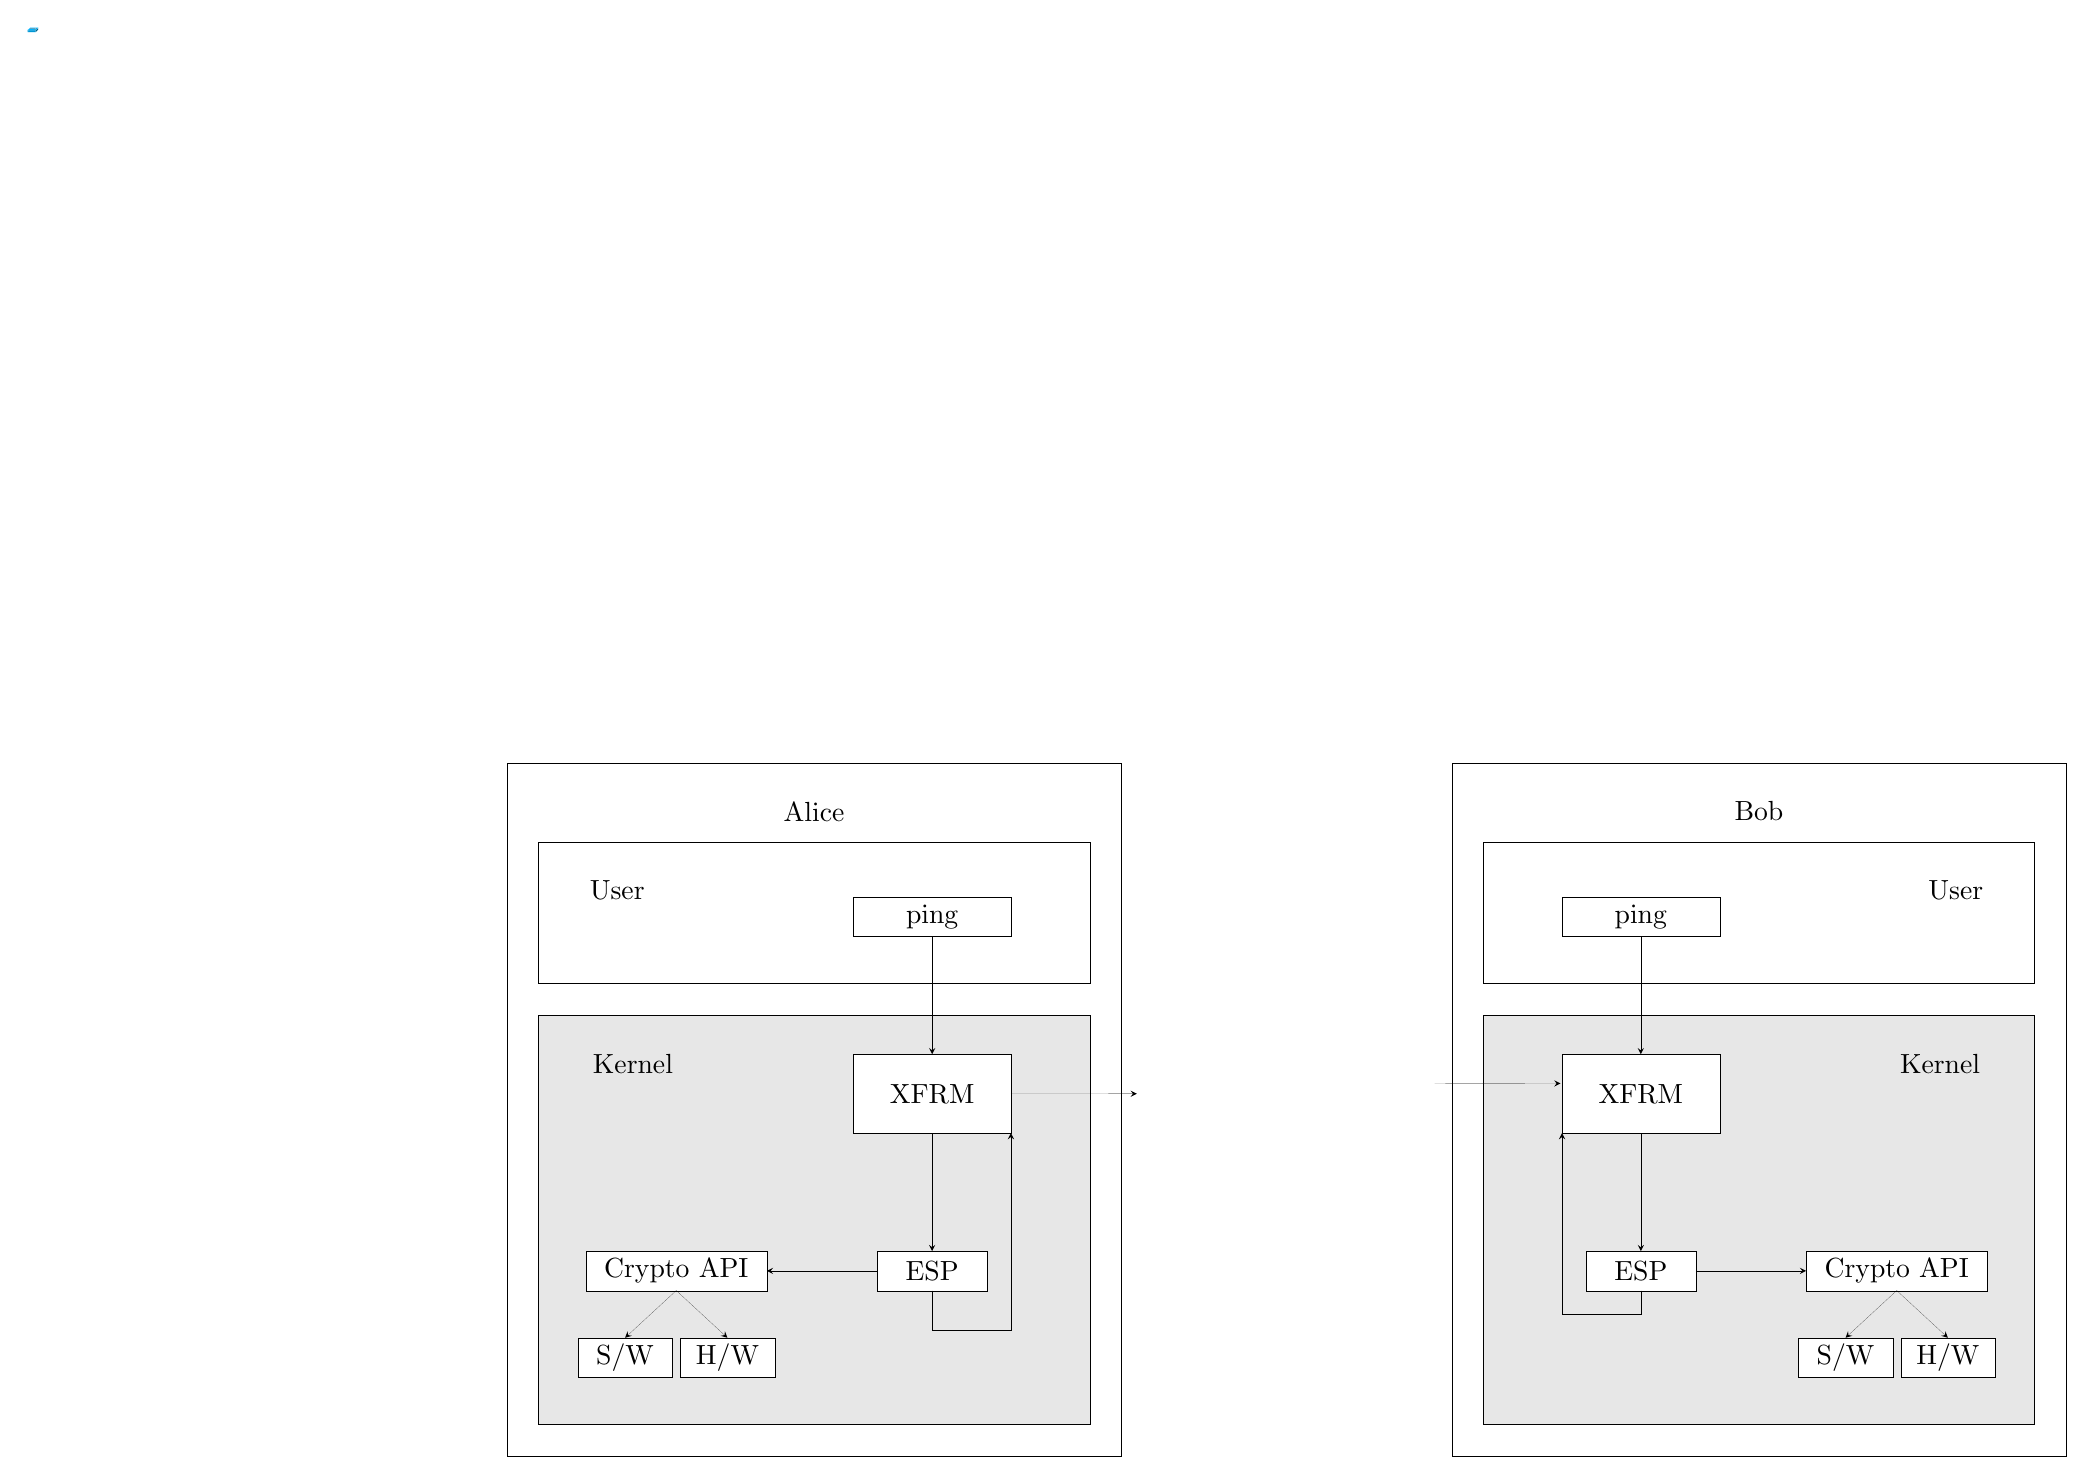
\begin{tikzpicture}
\pgftransformxscale{1.000000}
\pgftransformyscale{-1.000000}
\definecolor{dialinecolor}{rgb}{0.000000, 0.000000, 0.000000}
\pgfsetstrokecolor{dialinecolor}
\definecolor{dialinecolor}{rgb}{1.000000, 1.000000, 1.000000}
\pgfsetfillcolor{dialinecolor}
\pgfsetlinewidth{0.050000\du}
\pgfsetdash{}{0pt}
\pgfsetdash{}{0pt}
\pgfsetmiterjoin
\definecolor{dialinecolor}{rgb}{1.000000, 1.000000, 1.000000}
\pgfsetfillcolor{dialinecolor}
\fill (6.600000\du,9.800000\du)--(6.600000\du,10.800000\du)--(14.400000\du,10.800000\du)--(14.400000\du,9.800000\du)--cycle;
\definecolor{dialinecolor}{rgb}{0.000000, 0.000000, 0.000000}
\pgfsetstrokecolor{dialinecolor}
\draw (6.600000\du,9.800000\du)--(6.600000\du,10.800000\du)--(14.400000\du,10.800000\du)--(14.400000\du,9.800000\du)--cycle;
\pgfsetlinewidth{0.050000\du}
\pgfsetdash{}{0pt}
\pgfsetdash{}{0pt}
\pgfsetmiterjoin
\definecolor{dialinecolor}{rgb}{1.000000, 1.000000, 1.000000}
\pgfsetfillcolor{dialinecolor}
\fill (6.600000\du,9.800000\du)--(6.600000\du,18.600000\du)--(14.400000\du,18.600000\du)--(14.400000\du,9.800000\du)--cycle;
\definecolor{dialinecolor}{rgb}{0.000000, 0.000000, 0.000000}
\pgfsetstrokecolor{dialinecolor}
\draw (6.600000\du,9.800000\du)--(6.600000\du,18.600000\du)--(14.400000\du,18.600000\du)--(14.400000\du,9.800000\du)--cycle;
% setfont left to latex
\definecolor{dialinecolor}{rgb}{0.000000, 0.000000, 0.000000}
\pgfsetstrokecolor{dialinecolor}
\node at (10.500000\du,10.416250\du){Alice};
\pgfsetlinewidth{0.050000\du}
\pgfsetdash{}{0pt}
\pgfsetdash{}{0pt}
\pgfsetmiterjoin
\definecolor{dialinecolor}{rgb}{1.000000, 1.000000, 1.000000}
\pgfsetfillcolor{dialinecolor}
\fill (18.600000\du,9.800000\du)--(18.600000\du,10.800000\du)--(26.400000\du,10.800000\du)--(26.400000\du,9.800000\du)--cycle;
\definecolor{dialinecolor}{rgb}{0.000000, 0.000000, 0.000000}
\pgfsetstrokecolor{dialinecolor}
\draw (18.600000\du,9.800000\du)--(18.600000\du,10.800000\du)--(26.400000\du,10.800000\du)--(26.400000\du,9.800000\du)--cycle;
\pgfsetlinewidth{0.050000\du}
\pgfsetdash{}{0pt}
\pgfsetdash{}{0pt}
\pgfsetmiterjoin
\definecolor{dialinecolor}{rgb}{1.000000, 1.000000, 1.000000}
\pgfsetfillcolor{dialinecolor}
\fill (18.600000\du,9.800000\du)--(18.600000\du,18.600000\du)--(26.400000\du,18.600000\du)--(26.400000\du,9.800000\du)--cycle;
\definecolor{dialinecolor}{rgb}{0.000000, 0.000000, 0.000000}
\pgfsetstrokecolor{dialinecolor}
\draw (18.600000\du,9.800000\du)--(18.600000\du,18.600000\du)--(26.400000\du,18.600000\du)--(26.400000\du,9.800000\du)--cycle;
% setfont left to latex
\definecolor{dialinecolor}{rgb}{0.000000, 0.000000, 0.000000}
\pgfsetstrokecolor{dialinecolor}
\node at (22.500000\du,10.411344\du){Bob};
\pgfsetlinewidth{0.050000\du}
\pgfsetdash{}{0pt}
\pgfsetdash{}{0pt}
\pgfsetmiterjoin
\definecolor{dialinecolor}{rgb}{1.000000, 1.000000, 1.000000}
\pgfsetfillcolor{dialinecolor}
\fill (7.000000\du,13.000000\du)--(7.000000\du,14.000000\du)--(9.400000\du,14.000000\du)--(9.400000\du,13.000000\du)--cycle;
\definecolor{dialinecolor}{rgb}{0.000000, 0.000000, 0.000000}
\pgfsetstrokecolor{dialinecolor}
\draw (7.000000\du,13.000000\du)--(7.000000\du,14.000000\du)--(9.400000\du,14.000000\du)--(9.400000\du,13.000000\du)--cycle;
\pgfsetlinewidth{0.050000\du}
\pgfsetdash{}{0pt}
\pgfsetdash{}{0pt}
\pgfsetmiterjoin
\definecolor{dialinecolor}{rgb}{0.905882, 0.905882, 0.905882}
\pgfsetfillcolor{dialinecolor}
\fill (7.000000\du,13.000000\du)--(7.000000\du,18.200000\du)--(14.000000\du,18.200000\du)--(14.000000\du,13.000000\du)--cycle;
\definecolor{dialinecolor}{rgb}{0.000000, 0.000000, 0.000000}
\pgfsetstrokecolor{dialinecolor}
\draw (7.000000\du,13.000000\du)--(7.000000\du,18.200000\du)--(14.000000\du,18.200000\du)--(14.000000\du,13.000000\du)--cycle;
\pgfsetlinewidth{0.000000\du}
\pgfsetdash{}{0pt}
\pgfsetdash{}{0pt}
\pgfsetmiterjoin
\definecolor{dialinecolor}{rgb}{1.000000, 1.000000, 1.000000}
\pgfsetfillcolor{dialinecolor}
\fill (7.000000\du,10.800000\du)--(7.000000\du,11.800000\du)--(9.000000\du,11.800000\du)--(9.000000\du,10.800000\du)--cycle;
\definecolor{dialinecolor}{rgb}{1.000000, 1.000000, 1.000000}
\pgfsetstrokecolor{dialinecolor}
\draw (7.000000\du,10.800000\du)--(7.000000\du,11.800000\du)--(9.000000\du,11.800000\du)--(9.000000\du,10.800000\du)--cycle;
\pgfsetlinewidth{0.050000\du}
\pgfsetdash{}{0pt}
\pgfsetdash{}{0pt}
\pgfsetmiterjoin
\definecolor{dialinecolor}{rgb}{1.000000, 1.000000, 1.000000}
\pgfsetfillcolor{dialinecolor}
\fill (7.000000\du,10.800000\du)--(7.000000\du,12.600000\du)--(14.000000\du,12.600000\du)--(14.000000\du,10.800000\du)--cycle;
\definecolor{dialinecolor}{rgb}{0.000000, 0.000000, 0.000000}
\pgfsetstrokecolor{dialinecolor}
\draw (7.000000\du,10.800000\du)--(7.000000\du,12.600000\du)--(14.000000\du,12.600000\du)--(14.000000\du,10.800000\du)--cycle;
% setfont left to latex
\definecolor{dialinecolor}{rgb}{0.000000, 0.000000, 0.000000}
\pgfsetstrokecolor{dialinecolor}
\node at (8.000000\du,11.416250\du){User};
% setfont left to latex
\definecolor{dialinecolor}{rgb}{0.000000, 0.000000, 0.000000}
\pgfsetstrokecolor{dialinecolor}
\node at (8.200000\du,13.616250\du){Kernel};
\pgfsetlinewidth{0.050000\du}
\pgfsetdash{}{0pt}
\pgfsetdash{}{0pt}
\pgfsetmiterjoin
\definecolor{dialinecolor}{rgb}{1.000000, 1.000000, 1.000000}
\pgfsetfillcolor{dialinecolor}
\fill (23.600000\du,13.000000\du)--(23.600000\du,14.000000\du)--(26.000000\du,14.000000\du)--(26.000000\du,13.000000\du)--cycle;
\definecolor{dialinecolor}{rgb}{0.000000, 0.000000, 0.000000}
\pgfsetstrokecolor{dialinecolor}
\draw (23.600000\du,13.000000\du)--(23.600000\du,14.000000\du)--(26.000000\du,14.000000\du)--(26.000000\du,13.000000\du)--cycle;
\pgfsetlinewidth{0.050000\du}
\pgfsetdash{}{0pt}
\pgfsetdash{}{0pt}
\pgfsetmiterjoin
\definecolor{dialinecolor}{rgb}{0.905882, 0.905882, 0.905882}
\pgfsetfillcolor{dialinecolor}
\fill (19.000000\du,13.000000\du)--(19.000000\du,18.200000\du)--(26.000000\du,18.200000\du)--(26.000000\du,13.000000\du)--cycle;
\definecolor{dialinecolor}{rgb}{0.000000, 0.000000, 0.000000}
\pgfsetstrokecolor{dialinecolor}
\draw (19.000000\du,13.000000\du)--(19.000000\du,18.200000\du)--(26.000000\du,18.200000\du)--(26.000000\du,13.000000\du)--cycle;
\pgfsetlinewidth{0.000000\du}
\pgfsetdash{}{0pt}
\pgfsetdash{}{0pt}
\pgfsetmiterjoin
\definecolor{dialinecolor}{rgb}{1.000000, 1.000000, 1.000000}
\pgfsetfillcolor{dialinecolor}
\fill (24.000000\du,10.800000\du)--(24.000000\du,11.800000\du)--(26.000000\du,11.800000\du)--(26.000000\du,10.800000\du)--cycle;
\definecolor{dialinecolor}{rgb}{1.000000, 1.000000, 1.000000}
\pgfsetstrokecolor{dialinecolor}
\draw (24.000000\du,10.800000\du)--(24.000000\du,11.800000\du)--(26.000000\du,11.800000\du)--(26.000000\du,10.800000\du)--cycle;
\pgfsetlinewidth{0.050000\du}
\pgfsetdash{}{0pt}
\pgfsetdash{}{0pt}
\pgfsetmiterjoin
\definecolor{dialinecolor}{rgb}{1.000000, 1.000000, 1.000000}
\pgfsetfillcolor{dialinecolor}
\fill (19.000000\du,10.800000\du)--(19.000000\du,12.600000\du)--(26.000000\du,12.600000\du)--(26.000000\du,10.800000\du)--cycle;
\definecolor{dialinecolor}{rgb}{0.000000, 0.000000, 0.000000}
\pgfsetstrokecolor{dialinecolor}
\draw (19.000000\du,10.800000\du)--(19.000000\du,12.600000\du)--(26.000000\du,12.600000\du)--(26.000000\du,10.800000\du)--cycle;
% setfont left to latex
\definecolor{dialinecolor}{rgb}{0.000000, 0.000000, 0.000000}
\pgfsetstrokecolor{dialinecolor}
\node at (25.000000\du,11.416250\du){User};
% setfont left to latex
\definecolor{dialinecolor}{rgb}{0.000000, 0.000000, 0.000000}
\pgfsetstrokecolor{dialinecolor}
\node at (24.800000\du,13.616250\du){Kernel};
\pgfsetlinewidth{0.020000\du}
\pgfsetdash{}{0pt}
\pgfsetdash{}{0pt}
\pgfsetbuttcap
\pgfsetmiterjoin
\pgfsetlinewidth{0.000200\du}
\pgfsetbuttcap
\pgfsetmiterjoin
\pgfsetdash{}{0pt}
\definecolor{dialinecolor}{rgb}{0.000000, 0.588235, 0.831373}
\pgfsetfillcolor{dialinecolor}
\pgfpathmoveto{\pgfpoint{14.600000\du}{14.000632\du}}
\pgfpathlineto{\pgfpoint{14.600000\du}{14.731085\du}}
\pgfpathlineto{\pgfpoint{17.488279\du}{14.731085\du}}
\pgfpathlineto{\pgfpoint{17.488279\du}{14.000632\du}}
\pgfpathlineto{\pgfpoint{14.600000\du}{14.000632\du}}
\pgfusepath{fill}
\pgfsetbuttcap
\pgfsetmiterjoin
\pgfsetdash{}{0pt}
\definecolor{dialinecolor}{rgb}{0.666667, 0.901961, 1.000000}
\pgfsetstrokecolor{dialinecolor}
\pgfpathmoveto{\pgfpoint{14.600000\du}{14.000632\du}}
\pgfpathlineto{\pgfpoint{14.600000\du}{14.731085\du}}
\pgfpathlineto{\pgfpoint{17.488279\du}{14.731085\du}}
\pgfpathlineto{\pgfpoint{17.488279\du}{14.000632\du}}
\pgfpathlineto{\pgfpoint{14.600000\du}{14.000632\du}}
\pgfusepath{stroke}
\pgfsetbuttcap
\pgfsetmiterjoin
\pgfsetdash{}{0pt}
\definecolor{dialinecolor}{rgb}{0.000000, 0.352941, 0.501961}
\pgfsetfillcolor{dialinecolor}
\pgfpathmoveto{\pgfpoint{17.488279\du}{14.000632\du}}
\pgfpathlineto{\pgfpoint{18.381785\du}{13.140000\du}}
\pgfpathlineto{\pgfpoint{18.381785\du}{13.871110\du}}
\pgfpathlineto{\pgfpoint{17.488279\du}{14.731085\du}}
\pgfpathlineto{\pgfpoint{17.488279\du}{14.000632\du}}
\pgfusepath{fill}
\pgfsetbuttcap
\pgfsetmiterjoin
\pgfsetdash{}{0pt}
\definecolor{dialinecolor}{rgb}{0.666667, 0.901961, 1.000000}
\pgfsetstrokecolor{dialinecolor}
\pgfpathmoveto{\pgfpoint{17.488279\du}{14.000632\du}}
\pgfpathlineto{\pgfpoint{18.381785\du}{13.140000\du}}
\pgfpathlineto{\pgfpoint{18.381785\du}{13.871110\du}}
\pgfpathlineto{\pgfpoint{17.488279\du}{14.731085\du}}
\pgfpathlineto{\pgfpoint{17.488279\du}{14.000632\du}}
\pgfusepath{stroke}
\pgfsetbuttcap
\pgfsetmiterjoin
\pgfsetdash{}{0pt}
\definecolor{dialinecolor}{rgb}{0.000000, 0.705882, 1.000000}
\pgfsetfillcolor{dialinecolor}
\pgfpathmoveto{\pgfpoint{17.488279\du}{14.000632\du}}
\pgfpathlineto{\pgfpoint{18.381785\du}{13.140000\du}}
\pgfpathlineto{\pgfpoint{15.492848\du}{13.140000\du}}
\pgfpathlineto{\pgfpoint{14.600000\du}{14.000632\du}}
\pgfpathlineto{\pgfpoint{17.488279\du}{14.000632\du}}
\pgfusepath{fill}
\pgfsetbuttcap
\pgfsetmiterjoin
\pgfsetdash{}{0pt}
\definecolor{dialinecolor}{rgb}{0.666667, 0.901961, 1.000000}
\pgfsetstrokecolor{dialinecolor}
\pgfpathmoveto{\pgfpoint{17.488279\du}{14.000632\du}}
\pgfpathlineto{\pgfpoint{18.381785\du}{13.140000\du}}
\pgfpathlineto{\pgfpoint{15.492848\du}{13.140000\du}}
\pgfpathlineto{\pgfpoint{14.600000\du}{14.000632\du}}
\pgfpathlineto{\pgfpoint{17.488279\du}{14.000632\du}}
\pgfusepath{stroke}
\pgfsetbuttcap
\pgfsetmiterjoin
\pgfsetdash{}{0pt}
\definecolor{dialinecolor}{rgb}{0.000000, 0.000000, 0.000000}
\pgfsetfillcolor{dialinecolor}
\pgfpathmoveto{\pgfpoint{15.544789\du}{13.452300\du}}
\pgfpathlineto{\pgfpoint{15.388968\du}{13.608778\du}}
\pgfpathlineto{\pgfpoint{17.122067\du}{13.608778\du}}
\pgfpathlineto{\pgfpoint{16.989257\du}{13.739615\du}}
\pgfpathlineto{\pgfpoint{17.724970\du}{13.556838\du}}
\pgfpathlineto{\pgfpoint{17.358100\du}{13.374060\du}}
\pgfpathlineto{\pgfpoint{17.278545\du}{13.452300\du}}
\pgfpathlineto{\pgfpoint{15.544789\du}{13.452300\du}}
\pgfusepath{fill}
\pgfsetbuttcap
\pgfsetmiterjoin
\pgfsetdash{}{0pt}
\definecolor{dialinecolor}{rgb}{1.000000, 1.000000, 1.000000}
\pgfsetfillcolor{dialinecolor}
\pgfpathmoveto{\pgfpoint{15.571088\du}{13.478599\du}}
\pgfpathlineto{\pgfpoint{15.413294\du}{13.608778\du}}
\pgfpathlineto{\pgfpoint{17.147051\du}{13.608778\du}}
\pgfpathlineto{\pgfpoint{17.015556\du}{13.739615\du}}
\pgfpathlineto{\pgfpoint{17.724970\du}{13.583794\du}}
\pgfpathlineto{\pgfpoint{17.383084\du}{13.401017\du}}
\pgfpathlineto{\pgfpoint{17.278545\du}{13.478599\du}}
\pgfpathlineto{\pgfpoint{15.571088\du}{13.478599\du}}
\pgfusepath{fill}
\pgfsetlinewidth{0.020000\du}
\pgfsetdash{}{0pt}
\pgfsetdash{}{0pt}
\pgfsetmiterjoin
\definecolor{dialinecolor}{rgb}{1.000000, 1.000000, 1.000000}
\pgfsetfillcolor{dialinecolor}
\fill (11.000000\du,11.500000\du)--(11.000000\du,12.000000\du)--(13.000000\du,12.000000\du)--(13.000000\du,11.500000\du)--cycle;
\definecolor{dialinecolor}{rgb}{0.000000, 0.000000, 0.000000}
\pgfsetstrokecolor{dialinecolor}
\draw (11.000000\du,11.500000\du)--(11.000000\du,12.000000\du)--(13.000000\du,12.000000\du)--(13.000000\du,11.500000\du)--cycle;
% setfont left to latex
\definecolor{dialinecolor}{rgb}{0.000000, 0.000000, 0.000000}
\pgfsetstrokecolor{dialinecolor}
\node at (12.000000\du,11.750000\du){ping};
\pgfsetlinewidth{0.020000\du}
\pgfsetdash{}{0pt}
\pgfsetdash{}{0pt}
\pgfsetmiterjoin
\definecolor{dialinecolor}{rgb}{1.000000, 1.000000, 1.000000}
\pgfsetfillcolor{dialinecolor}
\fill (11.000000\du,13.500000\du)--(11.000000\du,14.500000\du)--(13.000000\du,14.500000\du)--(13.000000\du,13.500000\du)--cycle;
\definecolor{dialinecolor}{rgb}{0.000000, 0.000000, 0.000000}
\pgfsetstrokecolor{dialinecolor}
\draw (11.000000\du,13.500000\du)--(11.000000\du,14.500000\du)--(13.000000\du,14.500000\du)--(13.000000\du,13.500000\du)--cycle;
% setfont left to latex
\definecolor{dialinecolor}{rgb}{0.000000, 0.000000, 0.000000}
\pgfsetstrokecolor{dialinecolor}
\node at (12.000000\du,14.000000\du){XFRM};
\pgfsetlinewidth{0.020000\du}
\pgfsetdash{}{0pt}
\pgfsetdash{}{0pt}
\pgfsetmiterjoin
\definecolor{dialinecolor}{rgb}{1.000000, 1.000000, 1.000000}
\pgfsetfillcolor{dialinecolor}
\fill (11.300000\du,16.000000\du)--(11.300000\du,16.500000\du)--(12.700000\du,16.500000\du)--(12.700000\du,16.000000\du)--cycle;
\definecolor{dialinecolor}{rgb}{0.000000, 0.000000, 0.000000}
\pgfsetstrokecolor{dialinecolor}
\draw (11.300000\du,16.000000\du)--(11.300000\du,16.500000\du)--(12.700000\du,16.500000\du)--(12.700000\du,16.000000\du)--cycle;
% setfont left to latex
\definecolor{dialinecolor}{rgb}{0.000000, 0.000000, 0.000000}
\pgfsetstrokecolor{dialinecolor}
\node at (12.000000\du,16.250000\du){ESP};
\pgfsetlinewidth{0.020000\du}
\pgfsetdash{}{0pt}
\pgfsetdash{}{0pt}
\pgfsetmiterjoin
\definecolor{dialinecolor}{rgb}{1.000000, 1.000000, 1.000000}
\pgfsetfillcolor{dialinecolor}
\fill (7.600000\du,16.000000\du)--(7.600000\du,16.500000\du)--(9.900000\du,16.500000\du)--(9.900000\du,16.000000\du)--cycle;
\definecolor{dialinecolor}{rgb}{0.000000, 0.000000, 0.000000}
\pgfsetstrokecolor{dialinecolor}
\draw (7.600000\du,16.000000\du)--(7.600000\du,16.500000\du)--(9.900000\du,16.500000\du)--(9.900000\du,16.000000\du)--cycle;
% setfont left to latex
\definecolor{dialinecolor}{rgb}{0.000000, 0.000000, 0.000000}
\pgfsetstrokecolor{dialinecolor}
\node at (8.750000\du,16.250000\du){Crypto API};
\pgfsetlinewidth{0.020000\du}
\pgfsetdash{}{0pt}
\pgfsetdash{}{0pt}
\pgfsetmiterjoin
\definecolor{dialinecolor}{rgb}{1.000000, 1.000000, 1.000000}
\pgfsetfillcolor{dialinecolor}
\fill (7.500000\du,17.100000\du)--(7.500000\du,17.600000\du)--(8.700000\du,17.600000\du)--(8.700000\du,17.100000\du)--cycle;
\definecolor{dialinecolor}{rgb}{0.000000, 0.000000, 0.000000}
\pgfsetstrokecolor{dialinecolor}
\draw (7.500000\du,17.100000\du)--(7.500000\du,17.600000\du)--(8.700000\du,17.600000\du)--(8.700000\du,17.100000\du)--cycle;
% setfont left to latex
\definecolor{dialinecolor}{rgb}{0.000000, 0.000000, 0.000000}
\pgfsetstrokecolor{dialinecolor}
\node at (8.100000\du,17.350000\du){S/W};
\pgfsetlinewidth{0.020000\du}
\pgfsetdash{}{0pt}
\pgfsetdash{}{0pt}
\pgfsetmiterjoin
\definecolor{dialinecolor}{rgb}{1.000000, 1.000000, 1.000000}
\pgfsetfillcolor{dialinecolor}
\fill (8.800000\du,17.100000\du)--(8.800000\du,17.600000\du)--(10.000000\du,17.600000\du)--(10.000000\du,17.100000\du)--cycle;
\definecolor{dialinecolor}{rgb}{0.000000, 0.000000, 0.000000}
\pgfsetstrokecolor{dialinecolor}
\draw (8.800000\du,17.100000\du)--(8.800000\du,17.600000\du)--(10.000000\du,17.600000\du)--(10.000000\du,17.100000\du)--cycle;
% setfont left to latex
\definecolor{dialinecolor}{rgb}{0.000000, 0.000000, 0.000000}
\pgfsetstrokecolor{dialinecolor}
\node at (9.400000\du,17.350000\du){H/W};
\pgfsetlinewidth{0.020000\du}
\pgfsetdash{}{0pt}
\pgfsetdash{}{0pt}
\pgfsetbuttcap
{
\definecolor{dialinecolor}{rgb}{0.000000, 0.000000, 0.000000}
\pgfsetfillcolor{dialinecolor}
% was here!!!
\pgfsetarrowsend{stealth}
\definecolor{dialinecolor}{rgb}{0.000000, 0.000000, 0.000000}
\pgfsetstrokecolor{dialinecolor}
\draw (12.000000\du,14.500000\du)--(12.000000\du,16.000000\du);
}
\pgfsetlinewidth{0.020000\du}
\pgfsetdash{}{0pt}
\pgfsetdash{}{0pt}
\pgfsetbuttcap
{
\definecolor{dialinecolor}{rgb}{0.000000, 0.000000, 0.000000}
\pgfsetfillcolor{dialinecolor}
% was here!!!
\pgfsetarrowsend{stealth}
\definecolor{dialinecolor}{rgb}{0.000000, 0.000000, 0.000000}
\pgfsetstrokecolor{dialinecolor}
\draw (11.300000\du,16.250000\du)--(9.900000\du,16.250000\du);
}
\pgfsetlinewidth{0.020000\du}
\pgfsetdash{}{0pt}
\pgfsetdash{}{0pt}
\pgfsetbuttcap
{
\definecolor{dialinecolor}{rgb}{0.000000, 0.000000, 0.000000}
\pgfsetfillcolor{dialinecolor}
% was here!!!
\pgfsetarrowsend{stealth}
\definecolor{dialinecolor}{rgb}{0.000000, 0.000000, 0.000000}
\pgfsetstrokecolor{dialinecolor}
\draw (8.750000\du,16.500000\du)--(8.100000\du,17.100000\du);
}
\pgfsetlinewidth{0.020000\du}
\pgfsetdash{}{0pt}
\pgfsetdash{}{0pt}
\pgfsetbuttcap
{
\definecolor{dialinecolor}{rgb}{0.000000, 0.000000, 0.000000}
\pgfsetfillcolor{dialinecolor}
% was here!!!
\pgfsetarrowsend{stealth}
\definecolor{dialinecolor}{rgb}{0.000000, 0.000000, 0.000000}
\pgfsetstrokecolor{dialinecolor}
\draw (8.750000\du,16.500000\du)--(9.400000\du,17.100000\du);
}
\pgfsetlinewidth{0.020000\du}
\pgfsetdash{}{0pt}
\pgfsetdash{}{0pt}
\pgfsetbuttcap
{
\definecolor{dialinecolor}{rgb}{0.000000, 0.000000, 0.000000}
\pgfsetfillcolor{dialinecolor}
% was here!!!
\pgfsetarrowsend{stealth}
\definecolor{dialinecolor}{rgb}{0.000000, 0.000000, 0.000000}
\pgfsetstrokecolor{dialinecolor}
\draw (13.000000\du,14.000000\du)--(14.600000\du,14.000632\du);
}
\pgfsetlinewidth{0.020000\du}
\pgfsetdash{}{0pt}
\pgfsetdash{}{0pt}
\pgfsetbuttcap
{
\definecolor{dialinecolor}{rgb}{0.000000, 0.000000, 0.000000}
\pgfsetfillcolor{dialinecolor}
% was here!!!
\pgfsetarrowsend{stealth}
\definecolor{dialinecolor}{rgb}{0.000000, 0.000000, 0.000000}
\pgfsetstrokecolor{dialinecolor}
\draw (12.000000\du,12.000000\du)--(12.000000\du,13.500000\du);
}
\pgfsetlinewidth{0.020000\du}
\pgfsetdash{}{0pt}
\pgfsetdash{}{0pt}
\pgfsetmiterjoin
\pgfsetbuttcap
{
\definecolor{dialinecolor}{rgb}{0.000000, 0.000000, 0.000000}
\pgfsetfillcolor{dialinecolor}
% was here!!!
\pgfsetarrowsend{stealth}
{\pgfsetcornersarced{\pgfpoint{0.000000\du}{0.000000\du}}\definecolor{dialinecolor}{rgb}{0.000000, 0.000000, 0.000000}
\pgfsetstrokecolor{dialinecolor}
\draw (12.000000\du,16.500000\du)--(12.000000\du,17.000000\du)--(13.000000\du,17.000000\du)--(13.000000\du,14.500000\du);
}}
\pgfsetlinewidth{0.020000\du}
\pgfsetdash{}{0pt}
\pgfsetdash{}{0pt}
\pgfsetmiterjoin
\definecolor{dialinecolor}{rgb}{1.000000, 1.000000, 1.000000}
\pgfsetfillcolor{dialinecolor}
\fill (20.000000\du,11.500000\du)--(20.000000\du,12.000000\du)--(22.000000\du,12.000000\du)--(22.000000\du,11.500000\du)--cycle;
\definecolor{dialinecolor}{rgb}{0.000000, 0.000000, 0.000000}
\pgfsetstrokecolor{dialinecolor}
\draw (20.000000\du,11.500000\du)--(20.000000\du,12.000000\du)--(22.000000\du,12.000000\du)--(22.000000\du,11.500000\du)--cycle;
% setfont left to latex
\definecolor{dialinecolor}{rgb}{0.000000, 0.000000, 0.000000}
\pgfsetstrokecolor{dialinecolor}
\node at (21.000000\du,11.750000\du){ping};
\pgfsetlinewidth{0.020000\du}
\pgfsetdash{}{0pt}
\pgfsetdash{}{0pt}
\pgfsetmiterjoin
\definecolor{dialinecolor}{rgb}{1.000000, 1.000000, 1.000000}
\pgfsetfillcolor{dialinecolor}
\fill (20.000000\du,13.500000\du)--(20.000000\du,14.500000\du)--(22.000000\du,14.500000\du)--(22.000000\du,13.500000\du)--cycle;
\definecolor{dialinecolor}{rgb}{0.000000, 0.000000, 0.000000}
\pgfsetstrokecolor{dialinecolor}
\draw (20.000000\du,13.500000\du)--(20.000000\du,14.500000\du)--(22.000000\du,14.500000\du)--(22.000000\du,13.500000\du)--cycle;
% setfont left to latex
\definecolor{dialinecolor}{rgb}{0.000000, 0.000000, 0.000000}
\pgfsetstrokecolor{dialinecolor}
\node at (21.000000\du,14.000000\du){XFRM};
\pgfsetlinewidth{0.020000\du}
\pgfsetdash{}{0pt}
\pgfsetdash{}{0pt}
\pgfsetmiterjoin
\definecolor{dialinecolor}{rgb}{1.000000, 1.000000, 1.000000}
\pgfsetfillcolor{dialinecolor}
\fill (20.300000\du,16.000000\du)--(20.300000\du,16.500000\du)--(21.700000\du,16.500000\du)--(21.700000\du,16.000000\du)--cycle;
\definecolor{dialinecolor}{rgb}{0.000000, 0.000000, 0.000000}
\pgfsetstrokecolor{dialinecolor}
\draw (20.300000\du,16.000000\du)--(20.300000\du,16.500000\du)--(21.700000\du,16.500000\du)--(21.700000\du,16.000000\du)--cycle;
% setfont left to latex
\definecolor{dialinecolor}{rgb}{0.000000, 0.000000, 0.000000}
\pgfsetstrokecolor{dialinecolor}
\node at (21.000000\du,16.250000\du){ESP};
\pgfsetlinewidth{0.020000\du}
\pgfsetdash{}{0pt}
\pgfsetdash{}{0pt}
\pgfsetmiterjoin
\definecolor{dialinecolor}{rgb}{1.000000, 1.000000, 1.000000}
\pgfsetfillcolor{dialinecolor}
\fill (23.100000\du,16.000000\du)--(23.100000\du,16.500000\du)--(25.400000\du,16.500000\du)--(25.400000\du,16.000000\du)--cycle;
\definecolor{dialinecolor}{rgb}{0.000000, 0.000000, 0.000000}
\pgfsetstrokecolor{dialinecolor}
\draw (23.100000\du,16.000000\du)--(23.100000\du,16.500000\du)--(25.400000\du,16.500000\du)--(25.400000\du,16.000000\du)--cycle;
% setfont left to latex
\definecolor{dialinecolor}{rgb}{0.000000, 0.000000, 0.000000}
\pgfsetstrokecolor{dialinecolor}
\node at (24.250000\du,16.250000\du){Crypto API};
\pgfsetlinewidth{0.020000\du}
\pgfsetdash{}{0pt}
\pgfsetdash{}{0pt}
\pgfsetmiterjoin
\definecolor{dialinecolor}{rgb}{1.000000, 1.000000, 1.000000}
\pgfsetfillcolor{dialinecolor}
\fill (23.000000\du,17.100000\du)--(23.000000\du,17.600000\du)--(24.200000\du,17.600000\du)--(24.200000\du,17.100000\du)--cycle;
\definecolor{dialinecolor}{rgb}{0.000000, 0.000000, 0.000000}
\pgfsetstrokecolor{dialinecolor}
\draw (23.000000\du,17.100000\du)--(23.000000\du,17.600000\du)--(24.200000\du,17.600000\du)--(24.200000\du,17.100000\du)--cycle;
% setfont left to latex
\definecolor{dialinecolor}{rgb}{0.000000, 0.000000, 0.000000}
\pgfsetstrokecolor{dialinecolor}
\node at (23.600000\du,17.350000\du){S/W};
\pgfsetlinewidth{0.020000\du}
\pgfsetdash{}{0pt}
\pgfsetdash{}{0pt}
\pgfsetmiterjoin
\definecolor{dialinecolor}{rgb}{1.000000, 1.000000, 1.000000}
\pgfsetfillcolor{dialinecolor}
\fill (24.300000\du,17.100000\du)--(24.300000\du,17.600000\du)--(25.500000\du,17.600000\du)--(25.500000\du,17.100000\du)--cycle;
\definecolor{dialinecolor}{rgb}{0.000000, 0.000000, 0.000000}
\pgfsetstrokecolor{dialinecolor}
\draw (24.300000\du,17.100000\du)--(24.300000\du,17.600000\du)--(25.500000\du,17.600000\du)--(25.500000\du,17.100000\du)--cycle;
% setfont left to latex
\definecolor{dialinecolor}{rgb}{0.000000, 0.000000, 0.000000}
\pgfsetstrokecolor{dialinecolor}
\node at (24.900000\du,17.350000\du){H/W};
\pgfsetlinewidth{0.020000\du}
\pgfsetdash{}{0pt}
\pgfsetdash{}{0pt}
\pgfsetbuttcap
{
\definecolor{dialinecolor}{rgb}{0.000000, 0.000000, 0.000000}
\pgfsetfillcolor{dialinecolor}
% was here!!!
\pgfsetarrowsend{stealth}
\definecolor{dialinecolor}{rgb}{0.000000, 0.000000, 0.000000}
\pgfsetstrokecolor{dialinecolor}
\draw (21.000000\du,14.500000\du)--(21.000000\du,16.000000\du);
}
\pgfsetlinewidth{0.020000\du}
\pgfsetdash{}{0pt}
\pgfsetdash{}{0pt}
\pgfsetbuttcap
{
\definecolor{dialinecolor}{rgb}{0.000000, 0.000000, 0.000000}
\pgfsetfillcolor{dialinecolor}
% was here!!!
\pgfsetarrowsend{stealth}
\definecolor{dialinecolor}{rgb}{0.000000, 0.000000, 0.000000}
\pgfsetstrokecolor{dialinecolor}
\draw (21.700000\du,16.250000\du)--(23.100000\du,16.250000\du);
}
\pgfsetlinewidth{0.020000\du}
\pgfsetdash{}{0pt}
\pgfsetdash{}{0pt}
\pgfsetbuttcap
{
\definecolor{dialinecolor}{rgb}{0.000000, 0.000000, 0.000000}
\pgfsetfillcolor{dialinecolor}
% was here!!!
\pgfsetarrowsend{stealth}
\definecolor{dialinecolor}{rgb}{0.000000, 0.000000, 0.000000}
\pgfsetstrokecolor{dialinecolor}
\draw (24.250000\du,16.500000\du)--(23.600000\du,17.100000\du);
}
\pgfsetlinewidth{0.020000\du}
\pgfsetdash{}{0pt}
\pgfsetdash{}{0pt}
\pgfsetbuttcap
{
\definecolor{dialinecolor}{rgb}{0.000000, 0.000000, 0.000000}
\pgfsetfillcolor{dialinecolor}
% was here!!!
\pgfsetarrowsend{stealth}
\definecolor{dialinecolor}{rgb}{0.000000, 0.000000, 0.000000}
\pgfsetstrokecolor{dialinecolor}
\draw (24.250000\du,16.500000\du)--(24.900000\du,17.100000\du);
}
\pgfsetlinewidth{0.020000\du}
\pgfsetdash{}{0pt}
\pgfsetdash{}{0pt}
\pgfsetbuttcap
{
\definecolor{dialinecolor}{rgb}{0.000000, 0.000000, 0.000000}
\pgfsetfillcolor{dialinecolor}
% was here!!!
\pgfsetarrowsend{stealth}
\definecolor{dialinecolor}{rgb}{0.000000, 0.000000, 0.000000}
\pgfsetstrokecolor{dialinecolor}
\draw (18.381785\du,13.871110\du)--(19.980000\du,13.870000\du);
}
\pgfsetlinewidth{0.020000\du}
\pgfsetdash{}{0pt}
\pgfsetdash{}{0pt}
\pgfsetbuttcap
{
\definecolor{dialinecolor}{rgb}{0.000000, 0.000000, 0.000000}
\pgfsetfillcolor{dialinecolor}
% was here!!!
\pgfsetarrowsend{stealth}
\definecolor{dialinecolor}{rgb}{0.000000, 0.000000, 0.000000}
\pgfsetstrokecolor{dialinecolor}
\draw (21.000000\du,12.000000\du)--(21.000000\du,13.500000\du);
}
\pgfsetlinewidth{0.020000\du}
\pgfsetdash{}{0pt}
\pgfsetdash{}{0pt}
\pgfsetmiterjoin
\pgfsetbuttcap
{
\definecolor{dialinecolor}{rgb}{0.000000, 0.000000, 0.000000}
\pgfsetfillcolor{dialinecolor}
% was here!!!
\pgfsetarrowsend{stealth}
{\pgfsetcornersarced{\pgfpoint{0.000000\du}{0.000000\du}}\definecolor{dialinecolor}{rgb}{0.000000, 0.000000, 0.000000}
\pgfsetstrokecolor{dialinecolor}
\draw (21.000000\du,16.500000\du)--(21.000000\du,16.800000\du)--(20.000000\du,16.800000\du)--(20.000000\du,14.500000\du);
}}
\end{tikzpicture}

}
\caption{IPSec user/kernel space workflow, using \texttt{ping} as a test case.}
\label{fig:ipsec-workflow}
\end{figure}


\subsection{Linux drivers}
% Mention the fact that we use the assembly implementation of AES, not the generic C one.

\section{Offload}

\subsection{Silex engine}

\subsection{BA411E Driver}

\subsection{BA414E Driver}